\documentclass[a4, 14.49pt]{article}
\usepackage[english]{babel}
\usepackage[utf8]{inputenc}
\usepackage{graphicx}
\usepackage{fancyhdr}

\pagestyle{fancy}
\fancyhf{}
\lhead{Uppsala University}
\cfoot{\thepage}
\rfoot{Mohammadmahdi Amini}
\renewcommand{\headrulewidth}{0.5pt}
\renewcommand{\footrulewidth}{0.5pt}

\begin{document}

    \begin{titlepage}

        \begin{figure}
            \begin{minipage}{0.48\textwidth}
                \begin{flushleft}
                    
\includegraphics[scale=0.5]{Images/UU_LOGO.png}
                \end{flushleft}
            \end{minipage}\hfill
            \begin{minipage}{0.48\textwidth}
                \begin{flushright}
                    
\includegraphics[scale=0.5]{Images/UU_LOGO.png}
                \end{flushright}
            \end{minipage}
        \end{figure}

        \thispagestyle{fancy}

        \vspace{1in}

        \center

        \textsc{\large MASTER THESIS REPORT}

        \vspace{0.5in}

        \noindent\makebox[\linewidth]{\rule{\linewidth}{1.2pt}}
        \textsc{ \textbf{\large FenceX: High throughput scalable geofencing }}
        \noindent\makebox[\linewidth]{\rule{\linewidth}{1.2pt}}

        \vspace{0.5in}

        \begin{minipage}{0.48\textwidth}
            \begin{flushleft}
                \textit{Student:} \\
                Mohammadmahdi Amini \\
                mm7amini@gmail.com
            \end{flushleft}
        \end{minipage}
        \begin{minipage}{0.48\textwidth}
            \begin{flushright}
                \textit{Supervisor:} \\
                Salman Toor \\
                salman.toor@it.uu.se
            \end{flushright}
        \end{minipage}

        \vspace{2in}

        \textbf{\large Department of Information Technologies} \\

        \today

    \end{titlepage}

    \newpage

    \setcounter{page}{2}
    \tableofcontents
    \newpage

    \listoffigures
    \newpage

    \section{FenceX: High throughput scalable geofencing}

    \subsection{Note for readers}
    This document is structured in a top-down style. Which means initially the work is described with assumption that readers are familiar with all the mentioned technologies, patterns, buzz words and ... . And initially the number of references is low. Later in following sections, we tried to cover the used technologies, patterns and ... separately to the extend that context of thesis allows and most of the references are made in those sections.

    \section{Geofencing}
    TODO expand


    Geofencing essentially is checking whether a geosptial point is inside a geospatial shape or not. This can be done in two styles: push and poll.

    In poll style, a fence (geospatial shape) is queried against a database of coordinates (mover-id:geospatial point). The result is all of the coordinates that reside in the fence. This type of geofencing relies on geospatial indexing. So updating and querying the database of coordinates is CPU intensive.

    On the other hand in push style, fences are pretty much predefined. Whenever coordinates of a mover changes (a location update report arrives), an intersection check between a predefined fence and the newly reported coordinate will happen. Although no geosptial indexing is necessarily involved, the intersection checking operation is still CPU intensive.

    \begin{itemize}
        \item In poll style we have a \textbf{database of locations} and in push style, a \textbf{database of fences}.
        \item Poll style geofencing has an \textbf{on demand} nature while push style is of \textbf{real time} nature.
        \item Poll style fencing use cases: Taxi/police/ambulance dispatch. Disaster management.
        \item Push style fencing use cases: Elderly/Kid/Pet care. Gambling addiction management.
    \end{itemize}

    Please note that using poll/push terminology is an idea brought up in this thesis in order to facilitate conversations about different approaches to geofencing.

    \section{Problem statement}
    Both styles of geofencing are CPU intensive. Also, geofencing is usually implemented using databases interacting with disk and accessed over network. So a combination of natural computational latency and IO latency limits the overall throughput of systems providing geofencing services. This get worst in high load high scale use cases,
    As a remedy we can improve the computational aspect of the problem by improving the indexing algorithms. However, usually the IO latency is much more effective than operational burden. So the other approach to improve the throughput is using co-located in memory databases which do not interact with disk and are accessed through local network (localhost). In this thesis we focused on the later and tried to minimize the IO latency.

    \paragraph
    We decided to use co-located in memory databases to minimize IO. Everything will be fine until our systems faces an amount of load which can not be handled properly even after scaling up. At this stage we scale the system out and deploy more than one instance of the program. This will also help with resiliency of system; if one of the instances of program goes down or stop responding for some reason, the system can still keep serving with remaining available instances.

    \paragraph
    Until now we achieved high throughput, scalability and resiliency by minimizing IO latency and scaling the application out. Which means we ended up with a distributed system containing some components (instances of our application) that need to have same image of world, same data more precisely. The location updates or queries sent to the system by clients, can end up in any of the available instances due to load balancing. Otherwise there should be way to shard the data between instances and tell clients how to select the correct instance to which send a location update or query. We went to replication over sharding with hope of keeping clients and data management simple. So we need to some how make those instances have the same image of the world (same data) otherwise their results will be inconsistent.

    So far we have exchanged IO for the holly inconsistency issue of distributed systems. So the challenge is to keep the throughput, scalability and resiliency of geofencing system high while avoiding inconsistency among it's components.

    \subsection{functional requirements}
    Movers want their location reports be received by FenceX. This report contains the coordinate (latitude, longitude) at which mover was located when producing the report. A timestamp might be included in the report as well.

    Movers want their latest reported location to be available for being queried by their ID. (Movers want their latest reported location be memorised by system.)

    Users want to be able to send a geospatial shape (fence) to the system and in turn get movers (id:location) who are in the fence (according to their latest location report) = on demand fencing

    Users want to be able to create/update/remove/query a fence (geospatial shape) for each mover (by id).

    Movers expect each of the location reports to be checked against a potentially fence for them. Which mean for each location report for each mover, potentially a fence-point intersection should be
    calculated. The result of each intersection is if the reported coordinate located within the predefined fence. In case no fence is defined for a specific mover, no fence-point intersection should be calculated.


    \subsection{nonfunctional requirements}
    As a result of required system being a general geofencing provider, the required precision of system might vary based on the users and use cases. So FenceX should be able to ingest very high rates of location reports. Looking at potential use cases, in some the report rate could be like one report per mover every 1 minute and maximum of 1K active movers at the same time.
    Other cases might involve 1 location report per mover every 5 second with 1M active movers. So FenceX should have a very high capacity to handle load and stress.

    Since based on the use case, the required scalability of system may differ, the users of system should be able to tune the system in according to their needs. Or at least the fact that scalability requirements are not fixed over time should be factored in the design,

    Availability of FenceX should relay on modules so that if something goes wrong in one part of it, the other parts keep working. If FenceX stops receiving location reports, for instance, it should be still possible to query the saved locations by mover id and/or fence. In some cases it is acceptable to miss some location updates for some movers while in others, missing location reports is not tolerable due to high precision requirements.

    The time that takes for FenceX to answer a query by fence or calculate a fence-point intersection should not be a factor of the incoming load. In other words, the latency of those two operations should be reasonably low and should not increase as the load on the system increases. Such low latency will play a important role in the overall throughput of FenceX.


    Consistency level required for geofencing applications is not strong so eventual consistency will suffice. Once a location report has received, it might takes a fraction of time until the view of FenceX about corresponding mover changes. Before that, latest previously captured report and finalized view is valid and used. Same goes for predefined fences. So no need for distributed transactions or implementation of Saga as there is not much of intertwined that can go wrong.


    \section{Suggested solution}
    FenceX is a stream processing system designed and implemented into microservices. It can also be identified as a reactive distributed system that is applying event driven architecture for communication of its modules. These four big software architectural names are pretty much the same thing in the context of FenceX with their different being point of view. To avoid repeating same vocabulary over and over in this document, we use the terminology specific to each of these realms interchangeably on precisely when applicable. The listing below  illustrates words that refer to similar things but originate to different terminologies.

    \begin{itemize}
        \item[Microservice] microservice, service, operation, event processor,  processor, subscriber, publisher, module and subsystem.
        \item[Instance] instance, task
    \end{itemize}

    The exact meaning of each of the mentioned vocabulary and architectural styles will be discussed in following chapters. In case you are not familiar with any of them, please have a look at the corresponding chapters first.

    \section{overall system look}
    As you can see in the figure \ref{fig:logical-dfg}, FenceX has 6 operators. Some of them are stateful and backed by a state store and some of them are stateless.
    The exact details are as below in relation to state:

    \begin{itemize}
        \item[Stateful:] location-aggregate, fence-aggregate, location-fence-intersection
        \item[Stateless:] location-update-publisher (source), filter
    \end{itemize}

    \begin{figure}[ht]
        \caption{Logical data flow graph of FenceX}
        \label{fig:logical-dfg}
        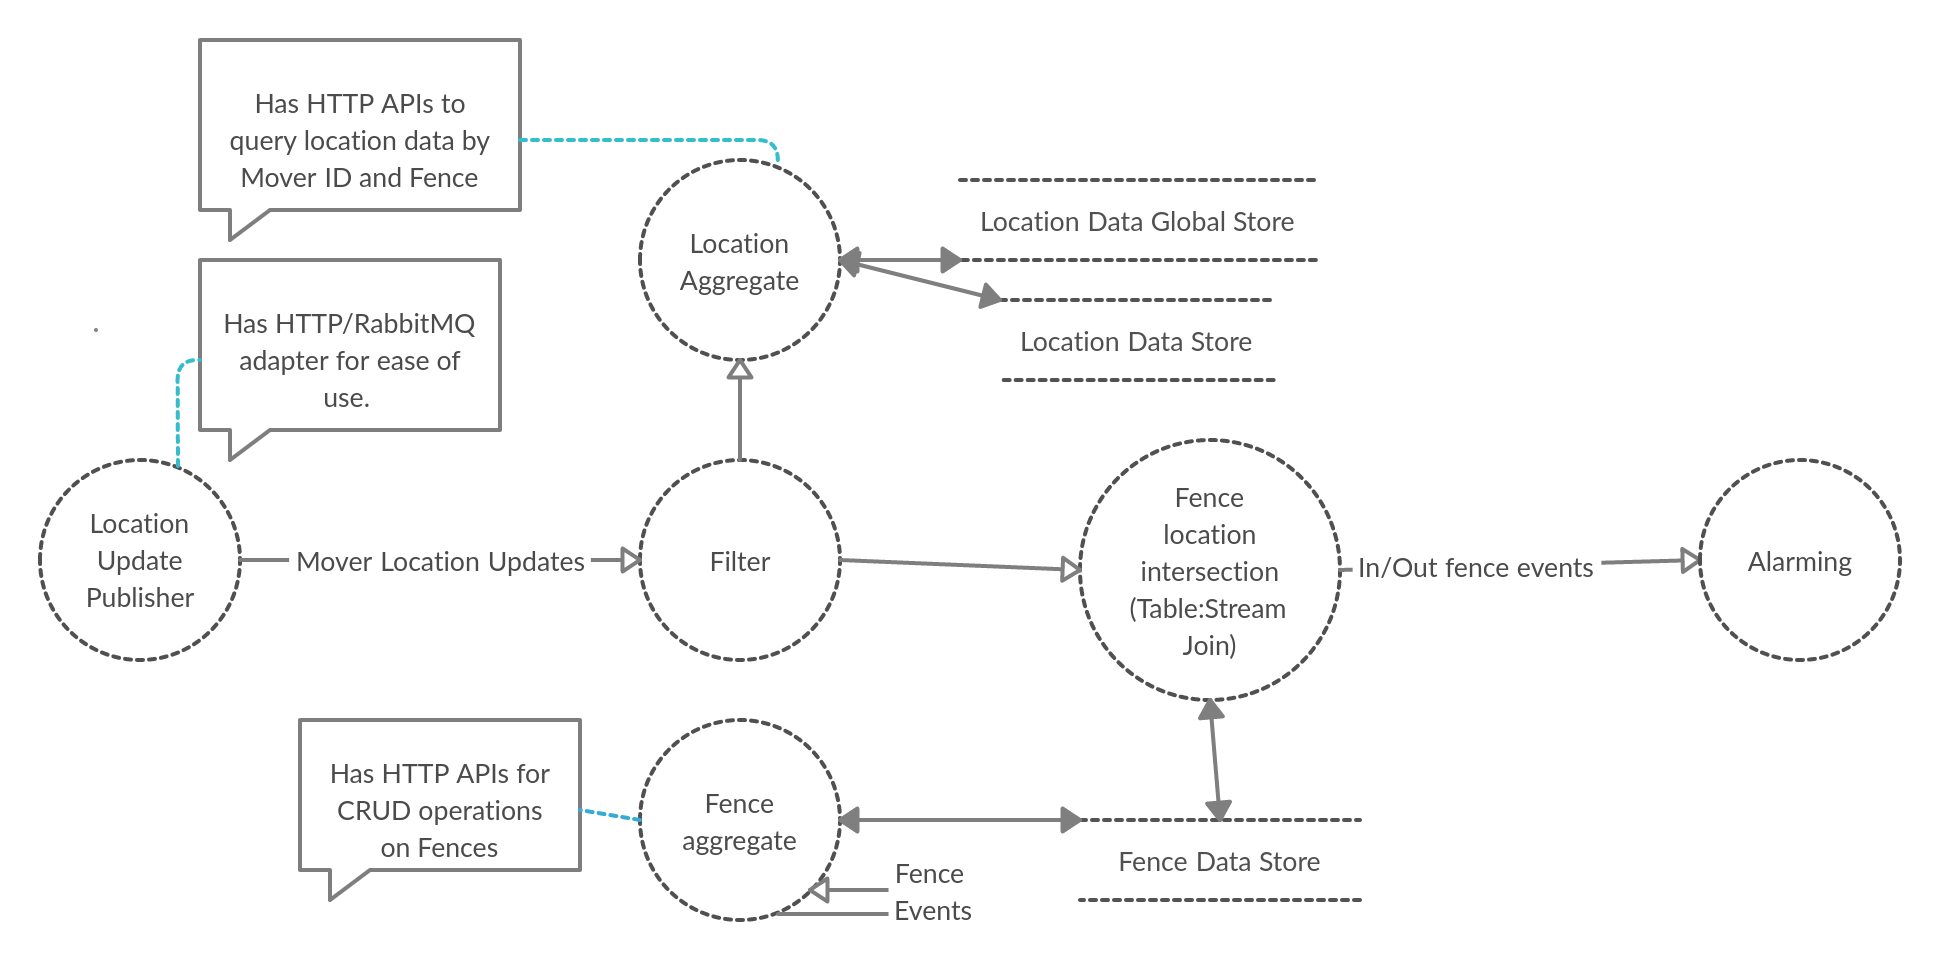
\includegraphics[scale=0.3]{Images/logical-data-flow-diagram.png}
        \centering
    \end{figure}

    \paragraph{location-update-publisher} plays the role of source in the FenceX stream processing pipe line. It has HTTP and RabbitMQ adaptors which is used by movers. Movers send messages or http requests in order report their latest location. Location-update-publisher turns each report into a event and publishes it into a kafka topic called \emph{location-updates}.

    \paragraph{filter}, as the name suggests, is responsible for avoiding not desired location updates to find their way further down in the stream. Checks can be against null values or invalid latitude/longitude.

    \paragraph{location-aggregate} is responsible for keeping a view of latest location of each mover by subscribing to the stream of location updates coming out of filter. It has a local database of mover-locations which applies geospatial index on the data. As a result, the query by fence is becomes possible. So location-aggregate is responsible for answering queries both by mover id and fence (geospatial shape).

    \paragraph{fence-aggregate} is responsible to keep track of predefined fences (for real time intersection scenarios).  It exposes HTTP APIs for CRUD operations. The fences are kept in an temporal KTable (kafka streams notion of table) and backed by a durable Kafka topic. In other words, each operation (CRUD) on each fence is initially a Kafka event which is later processed by fence-aggregate into a fence. The producer of those events is also fence-aggregate. In more technical terms, fence-aggregate is using event-sourcing architecture internally.

    \paragraph{fence-location-intersection} (join) has a view of predefined fences (managed by fence-aggregate) in shape of a key:value table. Key is id of mover for which the fence (value) is defined. fence-location-intersection is a join between that table and stream of location updates coming out of filter. Those location updates also has a key:value form. Key is the mover id and value is the reported location. And finally, the join operation is to check if the fence in table contains the location in the update. The result of this intersection will be events like mover X is (not) in the predefined fence.

    \paragraph{alarming} is responsible for responding to the events coming out of fence-location-intersection. Implementation of this operator is not withing boundaries of this thesis. So we won't describe its details.


    \subsection{Push and Poll leg}




    \nocite{*}
    \bibliography{sources}
    \bibliographystyle{IEEEtran}
\end{document}
